\documentclass[14pt]{extreport}
\usepackage[T1]{fontenc}
\usepackage[left=1in, right=1in, top=1in, bottom=1in]{geometry}
\usepackage{amsmath, amssymb, amsthm}
\usepackage{enumitem}
\usepackage{mathtools}
\usepackage{cancel}


\usepackage{bm}
% colored links
\usepackage{hyperref}
\hypersetup{
    colorlinks=true,
    linkcolor=blue,
    filecolor=magenta,      
    urlcolor=black!20!BurntOrange,
    }

% Inputting Python code
\usepackage[dvipsnames]{xcolor}
\definecolor{textblue}{rgb}{.2,.2,.7}
\definecolor{textred}{rgb}{0.54,0,0}
\definecolor{textgreen}{rgb}{0,0.43,0}
\usepackage{upquote}
\usepackage{listings}
\lstset{
    language=Python, 
    tabsize=4,
    basicstyle={\ttfamily},
    keywordstyle=\color{textblue},
    commentstyle=\color{textgreen},
    stringstyle=\color{textred},
    frame=none,
    columns=fullflexible,
    keepspaces=true,
    showstringspaces=false,
    xleftmargin=-15mm, % manual adjustment, figure out permanent solution
}

% Drawing figures
\usepackage{tikz}
\usetikzlibrary{matrix, positioning}
\usetikzlibrary{calc, shapes.symbols}

% Colored Boxes
\usepackage{tcolorbox}
\tcbuselibrary{skins,hooks}
\usetikzlibrary{shadows}
\usepackage{lipsum}

%Easy Numbering in case we add or remove questions
\newcounter{counter}
\newcommand{\Exercise}{Exercise \stepcounter{counter}\thecounter}

%Images
\usepackage{graphicx}
    \usepackage{subcaption}
    \usepackage{float}

%Formatting and Spacing
\setitemize[1]{noitemsep, parsep = 5pt, topsep = 5pt}
\setenumerate[1]{label = (\alph*), parsep = 1pt, topsep = 5pt}
\setlength\parindent{0pt}
\linespread{1.1}

%Cases Environment
\newlist{Cases}{enumerate}{3}
\setlist[Cases]{leftmargin = .25in, label = {Case \arabic*.}, topsep = 0.01in, itemsep = 0.04in, itemindent = .5in, parsep = 0in}

%Stats
\newcommand{\Cov}{\text{Cov}}
\newcommand{\trace}{\text{trace}}
\newcommand{\Normal}{\text{Normal}}
\newcommand{\var}[1]{\operatorname{var}\left(#1\right)}
\newcommand{\E}[2][]{\operatorname{E}_{#1}\left[#2\right]}
\renewcommand{\Pr}[2][]{\operatorname{P}_{#1}\left(#2\right)}

%Custom Title Fields
\newcommand{\lectTitle}{Exam 1 Review}
\newcommand{\lectTime}{March 7, 2022}
\newcommand{\lectClass}{Advanced Algorithms}
\newcommand{\lectClassInstructor}{Dana Randall}
\newcommand{\lectSection}{Spring 2024}
\newcommand{\lectAuthorName}{Sarthak Mohanty}


\title{
    \vspace{1.75in}
    \textbf{\lectClass:\\ \lectTitle}\\
    \vspace{0.1in}\large{\textit{\lectClassInstructor\ \lectSection}}
    \vspace{2in}
    \author{\textbf{Sarthak Mohanty}}
    \date{}
}

\begin{document}

\maketitle
\pagebreak

\subsection*{\Exercise}
    A three-way cut is a set of edges such that removing it from the graph yields three connected components. Modify the min-cut algorithm discussed in class to get a three-way min cut. Compute the probability of success of your design and discuss how to boost it to be 1 - $o(1)$.
    
    \vspace{3mm}
    \textit{Hint: Follow the process from class, taking special care near the end.}

\subsection*{\Exercise}
    \textit{(Navigating The Labyrinth)}
    The young maiden Ariadne is at the entrance of a simple labyrinth which branches in $m \ge 2$ corridors, as shown below. Unfortunately, she does not have her magic string with her! She knows the architect of the labyrinth, Daedalus, is somewhere in the labyrinth. She devises the following strategy to find him\footnote{This strategy is known as \textit{spiral search} and has been proven to be optimal. Looks like Ariadne was a Theory thread!}:

    \vspace{3mm}
    Continue until we reach $t$: execute cycles of steps, where the function determining the number of steps to walk before the $i$th turn starting from the origin is
    $$f(i) = \left(\frac{m}{m - 1}\right)^{i} \quad\forall i \ge 1$$
    What is the competitive ratio of this algorithm?

\begin{center}
    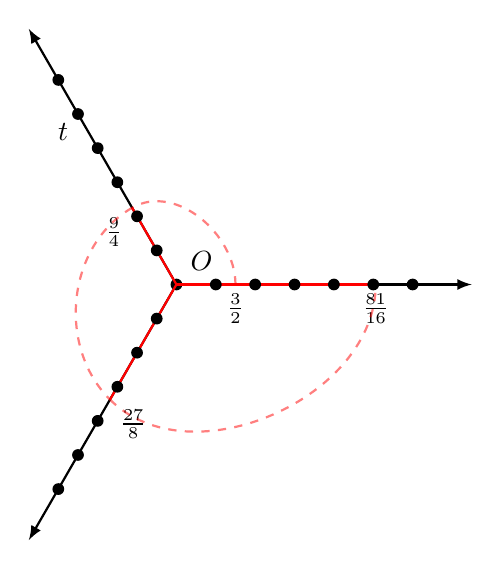
\begin{tikzpicture}[dot/.style={circle,fill,inner sep=1.5pt}, scale=0.5]
        \tikzset{>=latex}
        
        % Define the origin
        \node[dot,label=above right:$O$] (origin) at (0,0) {};
        
        % Calculate the ray length
        \pgfmathsetmacro{\raylength}{7.5}
        
        % Draw the rays at 120 degrees apart
        \foreach \a in {0,120,240} {
          \draw[thick,->] (origin) -- ++(\a:\raylength);
        }
        
        % Label
        \node at (120:5) [below left] {$t$};
        
        \node at (0:{3/2}) [below] {\small $\frac{3}{2}$};
        \node at (120:{9/4}) [below left] {\small $\frac{9}{4}$};
        \draw[red, thick] (120:0) -- (120:{9/4});
        \node at (240:{27/8}) [below right] {\small $\frac{27}{8}$};
        \draw[red, thick] (240:0) -- (240:{27/8});
        \node at (0:{81/16}) [below] {\small $\frac{81}{16}$};
        \draw[red, thick] (0:0) -- (0:{81/16});
        
        % Spiral connection with dotted lines
        \draw[red, thick, dashed, opacity=0.5] (0:{3/2}) to [out=90,in=30] (120:{9/4});
        \draw[red, thick, dashed, opacity=0.5] (120:{9/4}) to [out=210,in=135] (240:{27/8});
        \draw[red, thick, dashed, opacity=0.5] (240:{27/8}) to [out=-45,in=270] (0:{81/16});
        
        
        % Place dots on the rays
        % R ray
        \foreach \r in {1,...,6} {
          \node[dot] at (\r,0) {};
          % t ray
          \node[dot] at (120:\r) {};
          % H ray
          \node[dot] at (240:\r) {};
        }
    \end{tikzpicture}
\end{center}

\subsection*{\Exercise}
    \textit{(Potential Functions)} We discussed in class how potential functions were common motifs to help analyze online algorithms.
    
    \begin{enumerate}[label=(\alph*)]
        \item For an online algorithm $A$, let $c_A(\sigma)$ be the cost of the algorithm on the entire sequence and $c_A(i)$ be the cost on request $i$ (and similarly for $\text{OPT}$, the optimal offline algorithm). Prove the following. If for every request sequence $\sigma$ there exists a potential function $\Phi$ such that for all $1 \leq i \leq n$ we have
        $$
        c_A(i) + \Phi(i) - \Phi(i-1) \leq c \cdot c_{\text{OPT}}(i),
        $$ then $A$ is $c$-competitive.
        
        \item Consider the online problem \textsc{Read Into Buffer}: The task is to read an unknown-length non-empty string $s \in \Sigma^+$ of symbols into a buffer stored as contiguous array, one symbol at a time. The buffer must never be larger than $2|s|$ symbols. Reading a symbol has a basic cost of 1. When the currently allocated buffer is full, a new, larger array has to be allocated and the old contents must be copied, incurring a cost of 1 for each symbol already read. In other words, the cost for the $k$th symbol is either 1 (not full) or $k$ (full).
    
        \vspace{5mm}
        Devise an online algorithm for this problem and use a potential function to prove that its competitive ratio is at most 3.
    \end{enumerate}

\subsection*{\Exercise}
    In the context of the stable marriage problem, a loop is a sequence of distinct participants \( (X_1, Y_1, X_2, Y_2, \ldots, X_k, Y_k, X_1) \) with the following properties:
    \begin{enumerate}[label=\arabic*.]
        \item Each participant \( X_i \) prefers \( Y_i \) over \( Y_{i+1} \), with the exception that \( X_k \) prefers \( Y_k \) over \( Y_1 \).
        \item Each participant \( Y_i \) prefers \( X_{i+1} \) over \( X_i \), with the exception that \( Y_1 \) prefers \( X_1 \) over \( X_k \).
    \end{enumerate}
    Assess the accuracy of the following statement: A preference list containing a loop leads to the existence of at least one stable marriage.

\subsection*{\Exercise}
    Consider a scenario in the stable marriage problem involving $n$ men and $n$ women. Determine the \textit{exact} maximum number of proposals that could occur when running the Gale-Shapely algorithm.

\subsection*{\Exercise}
    Consider \textsc{FlushWhenFull} algorithm for paging: when a cache miss occurs and the entire cache is full, evict all pages from the cache. What is  the competitive ratio of \textsc{FlushWhenFull}?
    
\subsection*{\Exercise}    
    Consider adding the power of limited lookahead to an algorithm for paging. Namely, fix a constant $f \in \mathbb{N}$. Upon receiving the current page $p_i$, the algorithm also learns $p_{i+1}, p_{i+2}, \dots, p_{i+f}$. Recall that the best achievable competitive ratio for deterministic algorithms without lookahead is $k$. Can you improve on this bound with lookahead?

\subsection*{\Exercise}
    \textit{(Online Coloring)} We briefly covered coloring in our homework; now we will cover it in an online context. Our input sequence consists of the vertices $v_1, \ldots, v_n$ of an undirected graph $G = (\{v_1, \ldots, v_n\}, E)$. Together with each vertex $v_i$, we are given the list $E_i$ of all edges connecting $v_i$ to previously given vertices $v_1, \ldots, v_{i-1}$. Edges from $v_i$ to vertices $v_j$ with $j > i$ are only revealed once vertex $v_j$ is given. The number of edges and vertices in the graph is not known in advance.

    \vspace{5mm}
    When we are given $v_i$, we have to choose a color $c(v_i) \in \mathbb{N}$ for $v_i$ in such a way that no vertex adjacent to $v_i$ has color $c(v_i)$. As usual, this choice is final; we cannot change the color later on. We want to minimize the number of colors used. For an example, see Figure 1.

    \vspace{5mm}
    We want to show that there is no deterministic $c$-competitive algorithm for this problem for any constant $c$. For any constant number $2 \leq k \in \mathbb{N}$ of colors and any deterministic online algorithm $A$, devise a strategy for an adversary that satisfies the following requirements.
    \begin{itemize}
      \item The strategy always produces a forest $T_{A,k}$.
      \item The online algorithm $A$ uses at least $k$ colors on $T_{A,k}$.
    \end{itemize}
    Offline, every forest can be colored with 2 colors; therefore, this implies that $A$'s competitive ratio is at least $k/2$.

\subsection*{\Exercise\footnote{From Technische Universität Braunschweig.}}
    \textit{(Online Load Balancing)} We discussed load balancing quite a bit in the beginning of the semester. Here we consider a weighted variant. Suppose we receive a sequence of items, where $a_{i} \in (0, \infty)$ Moreover, we have a fixed number of $m$ bins with unlimited capacity. We have to pack each incoming item into a bin that we have to fix before the next item is given to us. As in load balancing, we want to minimize the total weight $W$ packed into the fullest bin.

    \vspace{5mm}
    We consider the following algorithm \textsc{GREEDY} for this problem. Initially, all bins are empty. On receiving the $i$th item $a_i$, \textsc{GREEDY} packs $a_i$ into the emptiest bin; ties are broken arbitrarily. For an example of the algorithm, refer to Figure 1.

\begin{figure}[H]
    \centering
    
\includegraphics[width=0.4\textwidth]{images/online_load_balancing_greedy.png}
    \caption{The packing that results from applying GREEDY to $m = 4$ bins and the input sequence $ (6, 7, 5, 11, 4, 5, 6) $. The quality of the solution produced by GREEDY is $W_G = 13$ (the fullest bin contains $7 + 6 = 13$ units of weight). The optimal solution has quality $W_O = 11$.}
    \label{fig:greedy_packing}
\end{figure}

\begin{enumerate}[label=(\arabic*)]
    \item Prove that \textsc{GREEDY} cannot be better than $ (2 - \frac{1}{m}) $-competitive. \textit{Hint: Consider a
    sequence that begins with small items and ends with a big item.}
    
    \item Prove that \textsc{GREEDY} is $ (2 - \frac{1}{m}) $-competitive. \textit{Hint: Consider the last item $a_T$ placed
    into the fullest bin and the value $W_G - a_T$.}
\end{enumerate}

\subsection*{\Exercise\footnote{Taken from CMU's 15-451/651 recitation.}}
    (\textit{k-wise Independent Hashing}) We can extend our definition of $k$-wise independence to hashing as well. A hash family $\mathcal{H}$ is \textit{k-wise independent} if for all $k$ distinct keys $x_1, x_2, \ldots, x_k \in \mathcal{U}$ and every set of $k$ values $v_1, v_2, \ldots, v_k \in \{0, 1, \ldots, m-1\}$, we have that $$ \Pr[h \in \mathcal{H}]{h(x_1) = v_1 \land h(x_2) = v_2 \land \ldots \land h(x_k) = v_k} = \frac{1}{m^k}$$
    Intuitively, this means that if you look at only up to $k$ keys, the hash family appears to hash them truly randomly.
    \begin{enumerate}
        \item Is this hash family from $U = \{a, b\}$ to $\{0, 1\}$ (i.e., $m = 2$) one-wise independent (i.e., uniform)? How about pairwise independent?
        $$ \arraycolsep=7pt
        \begin{array}{c|cc}
            & a & b \\
            \hline
            h_1 & 0 & 0 \\
            h_2 & 1 & 0 \\
        \end{array} $$
        
        \item Can you fill in the blanks in this hash family with values in $\{0, 1\}$ to make it pairwise independent? 3-wise independent?
        $$ \arraycolsep=7pt
        \begin{array}{c|ccc}
            & a & b & c \\
            \hline
            h_1 & 0 & 0 &  \\
            h_2 &  &  & 1 \\
            h_3 & 0 &  &  \\
            h_4 & 1 & 1 & 0 \\
        \end{array}  $$
    \end{enumerate}

\section*{\Exercise}
    Here we consider a classic 2-universal hash function. Consider a universe where the keys are $k$ bits long, so $U = 0, \dots, 2^{k} - 1$. For a matrix $ \bm{A} \in \{0, 1\}^{k \times n} $, define the function $ h_{A}(x) = \bm{A}\bm{x} $, where we do addition mod 2. Now consider the family of functions $ \mathcal{H} = \{h_{\bm{A}} : \bm{A} \in \{0, 1\}^{k \times n} \} $
    \begin{enumerate}
        \item Prove this function is 2-universal.
        \item How many random bits does it take to sample a random hash function from this family?
        \item \textit{(Optional)} What is the running time of $h$? How does it compare to, say, a binary search tree?
    \end{enumerate}

\section*{\Exercise}
    \textit{(Randall)} Construct an instance of the stable matching problem with 4 men and 4 women and a stable matching in which every man is matched to his least preferred woman.

\section*{\Exercise}
    \textit{(Randall)} Prove that in the output of the Traditional Dating Algorithm (when men propose) at most one man gets his last choice.

\section*{\Exercise}
    \textit{(Randall)} Recall that the woman optimal matching is the output of the TDA algorithm when women propose to men. Prove that an instance of the stable matching problem has exactly one stable matching if and only if the man optimal matching is equal to the woman optimal matching.

\pagebreak

\section*{Extra Practice}
    These are a collection of problems online I found interesting. I haven't drafted up solutions for these, and their relevance to the actual exam is undetermined.

\subsection*{\Exercise}
    Instead of searching for treasure on a line, consider the problem of searching for treasure on a 2-dimensional grid. The robot begins at the origin of $\mathbb{Z}^2$ and the treasure is located at some coordinate $(x, y) \in \mathbb{Z}^{2}$. The measure of distance is given by the Manhattan metric $\| (x,y) \| = |x| + |y|$. The robot has a compass and at each step can move north, south, east, or west one block. Design an algorithm for the robot to find the treasure on the grid. What is the competitive ratio of your algorithm? Can you improve the competitive ratio with another algorithm?

\subsection*{\Exercise}
    Consider the setting of the ski rental problem with rental cost $1$ and buying cost $b$, $b \in \mathbb{N}$. Instead of an adversary choosing a day $n \in \mathbb{N}$ when the weather is spoiled, this day is generated at random from distribution $p$. Design an optimal deterministic online algorithm for the following distributions $p$:
    
    \begin{enumerate}[label=(\alph*)]
        \item uniform distribution on $[n]$.
        \item geometric distribution on $\mathbb{N}$ with parameter $1/2$.
    \end{enumerate}

\subsection*{\Exercise}
    We are given a sequence of items of unknown weights $a_1, \ldots, a_n \in [0, 1]$ and want to assign these items to bins in an online fashion; however, the bins do not have limited capacity. In the \textsc{Bin Covering} problem, we want to \textit{maximize} the number of \textit{covered bins}, i.e., the number of bins that receive items of total weight at least 1. 
    
    \vspace{5mm} Find an online algorithm for \textsc{Bin Covering} with an absolute\footnote{We may have briefly mentioned this in class, but here ``absolute" just means replace the $\max$ in the definition with a $\sup$} competitive ratio of 2 and prove its competitive ratio. Prove that no deterministic online algorithm can have an absolute competitive ratio $ c < 2 $.

\subsection*{\Exercise\footnote{Taken from \href{https://www.ibr.cs.tu-bs.de/courses/ss18/oa/exercise_sheets/ex2.pdf}{here.}}}
    In this exercise, we consider the \textsc{List Update} Problem. Suppose that we are storing a set $S = {s_1, . . . , s_{n}}$ of values as unsorted linked list. Our input sequence consists of queries $s_{i} \in S$ that ask us to find a certain element in our list. In order to find an element, we iterate through the list starting from the front and return the element once we find it. Because iterating through our list takes time, we incur a cost of 1 for each element that we touch during the search. For example, searching for 2 in the list [1, 2, 3] costs two units, and searching for 2 in [2, 1, 3]
    costs just one unit.
    
    \vspace{5mm}
    After each query for an item $s_{i}$, we are allowed to move the item $s_{i}$ to any point closer to
    the front of the list; this exchange does not cost us anything. For example, if we search
    for 2 in the list [1, 4, 2, 3], we can change the list to [2, 1, 4, 3], [1, 2, 4, 3] or [1, 4, 2, 3] after finding 2 for a total cost of three units.
    
    \vspace{5mm}
    Our goal is to devise an online algorithm for this problem; after each request, the algorithm has to decide where to move the requested item. Intuitively speaking, we want our
    algorithm to maintain its list such that frequently requested elements are closer to the
    front than less frequently requested elements.
    \begin{enumerate}
        \item The algorithm \textsc{FrequencyCount} maintains a frequency count for each element that is incremented each time the element is requested. After each request, it moves the requested item such that the list is in nonincreasing order of frequency count. Prove that \textsc{FrequencyCount} is not $c$-competitive for any constant $c$.
        \item Now consider the \textsc{MoveToFront} algorithm for the List Update Problem. After each request $s_{i}$, the algorithm moves the requested item $s_{i}$ to the front of the list. For example, after searching for 2 in [1, 4, 2, 3], the list becomes [2, 1, 4, 3].

        \vspace{5mm}
        \textit{Hint:} Use the number of inversions in \textsc{MoveToFront}’s list with respect to OPT’s list after request $i$ as a potential function $\Phi(i)$. An inversion is a pair $(x, y)$ of elements such that $x$ comes before $y$ in \textsc{MoveToFront}’s list, but after $y$ in OPT’s list.
        
        \vspace{3mm}
        In order to prove $c_{\text{MTF}}(i) + \Phi(i) - \Phi(i - 1) \leq 2c_{\text{OPT}}(i)$ for a request $s_i$, consider the number of items $k$ that come before $s_i$ in both OPT’s and \textsc{MoveToFront}’s list and the number of items $\ell$ that come before $s_i$ in \textsc{MoveToFront}’s list but after $s_i$ in OPT’s list.
    \end{enumerate}
    
\end{document}

Construct an instance of the stable matching problem with 4 men and 4 women and a stable matching in which every man is matched to his least preferred woman.

Prove that in the output of the Traditional Dating Algorithm (when men propose) at most one man gets his last choice.

Recall that the woman optimal matching is the output of the TDA algorithm when women propose to men. Prove that an instance of the stable matching problem has exactly one stable matching if and only if the man optimal matching is equal to the woman optimal matching.

https://core.ac.uk/reader/216306720

https://www.cs.toronto.edu/~bor/2420s19/papers/draft-ch1-8.pdf

https://www.ibr.cs.tu-bs.de/courses/ss18/oa/exercise_sheets/ex3.pdf